%% Template para dissertacao/tese na classe UFBAthesis
%% versao 1.0
%% (c) 2005 Paulo G. S. Fonseca
%% (c) 2012 Antonio Terceiro
%% (c) 2014 Christina von Flach
%% www.dcc.ufba.br/~flach/ufbathesis

%% Carrega a classe ufbathesis
%% Opcoes: * Idiomas
%%           pt   - portugues (padrao)
%%           en   - ingles
%%         * Tipo do Texto
%%           bsc  - para monografias de graduacao
%%           msc  - para dissertacoes de mestrado (padrao)
%%           qual - exame de qualificacao de mestrado
%%           prop - exame de qualificacao de doutorado
%%           phd  - para teses de doutorado
%%         * Media
%%           scr  - para versao eletronica (PDF) / consulte o guia do usuario
%%         * Estilo
%%           classic - estilo original a la TAOCP (deprecated) - apesar de deprecated, manter esse.
%%           std     - novo estilo a la CUP (padrao)
%%         * Paginacao
%%           oneside - para impressao em face unica
%%           twoside - para impressao em frente e verso (padrao)

% Aten��o: Manter 'classic' na declaracao abaixo:
\documentclass[qual, classic, a4paper]{ufbathesis}

%% Preambulo:
\usepackage[utf8]{inputenc}
\usepackage{graphicx}
\usepackage{lipsum}
\usepackage{hyphenat}
\usepackage[usenames, dvipsnames, table]{xcolor}
\usepackage{booktabs}
\usepackage{pifont}
\usepackage{multirow}
\usepackage{listings} 
\usepackage{colortbl}
\usepackage{xfrac}
\usepackage[FIGTOPCAP]{subfigure}
\usepackage[printonlyused, withpage]{acronym}

% Universidade
\university{Universidade Federal da Bahia}

% Endereco (cidade)
\address{Salvador}

% Instituto ou Centro Academico
\institute{Instituto de Matem\'{a}tica}

% Nome da biblioteca - usado na ficha catalografica
\library{Biblioteca Reitor Mac\^{e}do Costa}

% Programa de pos-graduacao
\program{Programa de P\'{o}s-Gradua\c{c}\~{a}o em Ci\^{e}ncia da Computa\c{c}\~{a}o}

% Area de titulacao
\majorfield{Ci\^{e}ncia da Computa\c{c}\~{a}o}

% Titulo da dissertacao
\title{Detecção de mudanças de conceito em fluxos de dados não estacionários}

% Data da defesa
% e.g. \date{19 de fevereiro de 2013}
\date{19 de Julho de 2018}
% e.g. \defenseyear{2013}
\defenseyear{2018}

% Autor
% e.g. \author{Jose da Silva}
\author{Ruivaldo Azevedo Lobão Neto}

% Orientador(a)
% Opcao: [f] - para orientador do sexo feminino
% e.g. \adviser[f]{Profa. Dra. Maria Santos}
%\adviser{Ricardo Araújo Rios}
\adviser{***}

% Orientador(a)
% Opcao: [f] - para orientador do sexo feminino
% e.g. \coadviser{Prof. Dr. Pedro Pedreira}
% Comente se nao ha co-orientador
%\coadviser{Nome Completo do CO-ORIENTADOR}

%% Inicio do documento
\begin{document}

\pgcompfrontpage

%% Parte pre-textual
\frontmatter

\pgcomppresentationpage


%%%%%%%%%%%%%%%%%%%%%
% Resumo em Portugues
%%%%%%%%%%%%%%%%%%%%%

\resumo
O aprendizado a partir de fluxos de dados (aprendizagem incremental) tem crescido como foco de pesquisa, graças a existência de problemas práticos e desafios em aberto.
Dentre estes, está a detecção de mudanças de conceito, fenômeno que ocorre quando a distribução dos dados é alterada, tornando o modelo vigente impreciso ou obsoleto.
Neste trabalho, propomos uma nova técnica para detecção de mudanças de conceito.

% Palavras-chave do resumo em Portugues
\begin{keywords}
Mudança de conceito, detecção de mudanças, aprendizagem adaptativa, fluxos de dados.
\end{keywords}

%%%%%%%%%%%%%%%%%%%
% Resumo em Ingles
%%%%%%%%%%%%%%%%%%%

\abstract
Learning from data streams (incremental learning) is increasing as a research focus, due to the existence of practical problems and open challenges. Among which, is the detection of concept drift, a phenomenon that happens when the data distribution is altered, making the model inaccurate or obsolete. In this work, we propose a novel technic to detect concept drifts.

% Palavras-chave do resumo em Ingles
\begin{keywords}
Concept drift, change detection, adaptive learning, data streams.
\end{keywords}

%%%%%%%%%%%%%%%%%%%
% Sumario / Indice
%%%%%%%%%%%%%%%%%%%

% Comente para ocultar
\tableofcontents

% Lista de figuras
% Comente para ocultar
%\listoffigures

% Lista de tabelas
% Comente para ocultar
%\listoftables

%\chapter*{Lista de Siglas}

% Sintaxe da lista de acordo com a documentação do pacote `acronym'
% documentação: http://mirror.unl.edu/ctan/macros/latex/contrib/acronym/acronym.pdf
%\begin{acronym}[PGCOMP]
%    \acro{PGCOMP}{Programa de Pós-Graduação em Ciência da Computação}
    %\acro{CNPq}{Conselho Nacional de Desenvolvimento Científico e Tecnológico}
%\end{acronym}

%% Parte textual
\mainmatter

% Eh aconselhavel criar cada capitulo em um arquivo separado, digamos
% "capitulo1.tex", "capitulo2.tex", ... "capituloN.tex" e depois
% inclui-los com:
% \include{capitulo1}
% \include{capitulo2}
% ...
% \include{capituloN}
%
% Importante: 
% Use \xchapter{}{} ao inves de \chapter{}; se n�o quiser colocar texto antes do inicio do capitulo, use \xchapter{texto}{}.

% \xchapter{Introdu\c{c}\~{a}o}{Este eh o primeiro cap\'{\i}tulo, onde eu conto toda a historia deste trabalho, o problema, a solu\c{c}\~{a}o, etc.}

% É recomendável utilizar `\acresetall' no início de cada capítulo para reiníciar o contator de referências às siglas.
% \acresetall 


%\section{Se\c{c}\~{a}o}
%Trabalho do  \ac{PGCOMP}. Bolsa do \ac{CNPq}.

%\begin{figure}[h]
%Figure
%\caption{As siglas também funcionam nas legendas, seja na forma de sigla \ac{CNPq}, seja na forma completa \acf{PGCOMP}.}
%\end{figure}

%\lipsum

%\subsection{Uma Subse\c{c}\~{a}o}
%\acresetall
%Texto para mostrar como o \verb|\acresetall| funciona \ac{CNPq}, \ac{PGCOMP}. Ele reseta os contadoes e faz a sigla %aparecer na forma estendida novamente.

%\subsection{Outra Subse\c{c}\~{a}o}

%Texto  \acf{CNPq}, \acf{PGCOMP}.

\xchapter{Revis\~{a}o Bibliogr\'{a}fica}{}

\subsection{Introdução}

A extração de informações úteis a partir de grandes conjuntos de dados é uma tarefa desafiadora para os pesquisadores.
Os algoritmos de aprendizagem de máquina baseados em fluxos de dados contínuos (FCDs) atuam em um contexto diferente dos algoritmos tradicionais, 
devido a natureza dinâmica das FCDs.
Esses algoritmos devem se adaptar às constantes mudanças de distribuição dos dados, para não se tornarem imprecisos ou obsoletos.

Portanto, a atividade de Detecção de Novidades (DN) - \textit{Concept Drift} - é essencial para o bom funcionamento dessas técnicas. A atividade de DN permite identificar o surgimento de novos conceitos e mudanças em conceitos existentes, possibilitando a atualização do modelo de decisão. Novas técnicas de aprendizado ativo têm sido exploradas com o objetivo de aprimorar o processo de classificação e identificação de mudanças de conceito. 

\subsection{Fluxos Contínuos de Dados}

Fluxos Contínuos de Dados (FCDs) podem ser definidos como sequências contínuas de dados, de tamanho ilimitado, sem ordem definida e de alta frequência \cite{Babcock:2002:MID:543613.543615}. Novos algoritmos têm sido desenvolvidos para trabalhar com fluxos desse tipo, por exemplo: CLAM \cite{malkhateeb} e OLINDDA \cite{Spinosa:2009:NDA:1551768.1551770}. O desenvolvimento de algoritmos de aprendizado para esses cenários é uma tarefa custosa, pois devem lidar com sequências de dados geradas de forma contínua, em alta velocidade e cuja distribuição pode sofrer alterações ao longo do tempo \cite{Gama:2014:survey}.

Os avanços recentes em hardware e software permitiram a aquisição de dados em maior escala, o que caracteriza ambientes dinâmicos, enquanto bases de dados tradicionais supõem cenários estacionários. O contínuo avanço das tecnologias, surgiram diversas aplicações do mundo real baseadas em fluxos contínuos de dados: 

\begin{itemize}
    \item \textbf{Sistemas de Segurança}: monitoramento contínuo através de imagens ou outros sensores para identificação de intrusos;

    \item \textbf{Redes de Computadores}: análise do tráfego de rede, monitorando pacotes distoantes, além de realizar a detecção de invasores;

    \item \textbf{Mercado Financeiro}: análise de dados e estatísticas da bolsa de valores, produzindo informações importantes para investidores. Outra vertente é a aplicação na detecção de fraudes;

    \item \textbf{Medicina}: aprimoramento do modelo de detecção de determinada doença a partir das análises e resultados de novos casos.
\end{itemize}

Conforme \cite{Gama:2014:survey}, as principais características dos fluxos contínuos de dados são:

\begin{itemize}
    \item \textbf{Contínuos}: Elementos que compõem os dados são recebidos de forma continuada;

    \item \textbf{Não estacionário}: Distribuição de probabilidade sofre alterações o longo do tempo;

    \item \textbf{Potencialmente Infinitos}: Os fluxos são potencionalmente infinitos, o que impede o completo armazenamento em memória.
\end{itemize}

Essas propriedades inviabilizam a aplicação dos algoritmos tradicionais de mineração de dados (MD) e aprendizagem de máquina, a fluxos de dados contínuos.

Mudança de conceito (\textit{concept drift}) é uma mudança na distribuição dos dados utilizados para construção do modelo - definição dos conceitos (classes) - durante a execução da aplicação. A figura \ref{fig1} representa um caso clássico de mudança de conceito: a alteração do perfil de compra do cliente ao longo do tempo.

\begin{figure}[htbp]
    \begin{center}
      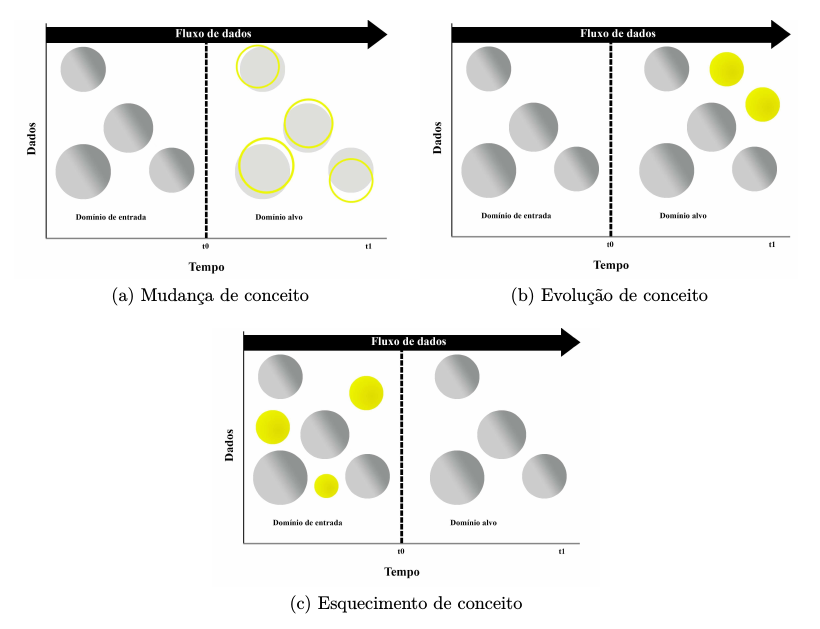
\includegraphics[scale=0.4]{001.png}
    \caption{Mudança de conceito - Exemplo: Perfil de Compra}
    \label{fig1}
    \end{center}
\end{figure}

A evolução de conceito (\textit{concept evolution}) caracteriza-se pela aparição de novas classes, diferente das classes conhecidas. Essa nova classe representa uma evolução, por exemplo, um novo interesse do cliente. Para que seja possível aprimorar modelos baseados em FCDs, é necessário esquecer conceitos desatualizados ou obsoletos, que apenas ocupam espaço e degradam o resultado das predições \cite{Abdallah}.

\subsection{Algoritmos de classificação e FCDs}

Algoritmos de classificação aplicados a FCDs permitem predizer, com alta precisão, a classe de novos exemplos obtidos a partir do fluxo. 
Durante o aprendizado supervisionado, um conjunto de dados previamente rotulado é fornecido ao algoritmo, para construção do modelo. A construção do modelo possibilita inferir a classe de novos exemplos que venham a ser encontrados. É importante que o modelo seja constantemente atualizado (evolua), para que contemple e classifique de forma correta novas distribuições de dados.

Dentre os algoritmos de classificação para cenários tradicionais (informação em lote, \textit{batch}), estão: árvores de decisão, SVM e Naive Bayes. Esses algoritmos são aplicados em ambientes estacionários, isto é, em ambientes em que o modelo de decisão não requer atualizações e o algoritmo pode considerar que todos dados necessários podem ser armazenados em memória.

Entretanto, o aprendizado de novos conceitos a partir de fluxos contínuos de dados ocorre de forma signitificamente diferente do modelo tradicional, estático. Para lidar 
% Aprender novos conceitos a partir de Ćuxos contínuos de dados, de forma a atualizar o modelo de decisão constantemente, é signiĄcativamente diferente do aprendizado tradicional, no qual uma vez criado o modelo, este não se altera ao longo do tempo. Vários algoritmos projetados para cenários estáticos tem sido adaptados e novos algoritmos estão sendo desenvolvidos para atuar em cenários dinâmicos. 


%hline
%\end{tabular}
%\end{center}
%\label{default-table2}
%\end{table}%

%\xchapter{Outro cap\'{\i}tulo}{} %sem preambulo
%\lipsum


%% Parte pos-textual
\backmatter

% Bibliografia
% � aconselh�vel utilizar o BibTeX a partir de um arquivo, digamos "biblio.bib".
% Para ajuda na cria��o do arquivo .bib e utiliza��o do BibTeX, recorra ao
% BibTeXpress em www.cin.ufpe.br/~paguso/bibtexpress
\bibliographystyle{abntex2-alf}
\bibliography{biblio}

% Apendices
% Comente se naoo houver apendices
%\appendix

%\xchapter{Exemplo de Ap\^endice}{} %sem preambulo
%\lipsum
% Eh aconselhavel criar cada apendice em um arquivo separado, digamos
% "apendice1.tex", "apendice.tex", ... "apendiceM.tex" e depois
% inclui--los com:
% \include{apendice1}
% \include{apendice2}
% ...
% \include{apendiceM}

%% Fim do documento
\end{document}
%------------------------------------------------------------------------------------------%
